\documentclass[a4paper,oneside,12pt]{article}
\usepackage[utf8]{inputenc}
\usepackage{dcolumn}
\usepackage[spanish]{babel}

\usepackage{graphicx}

\begin{document}

\pagenumbering{arabic}

\title{CRefactory}
\author{Baglivo Nicol\'as C\'esar \and Costa Federico Daniel \and Perera Nicanor Gonzalo \and Szeinfeld Matias Ezequiel \and Tarragona Juan Pablo}
\date{\today}
\maketitle

\tableofcontents

\newpage

\section{Organizaci\'on del documento}
En la secci\'on~\ref{sec:intro} se pretende poner en contexto al lector, introduciendo de manera breve y consisa algunos conceptos necesarios para luego explicar cual es la motivaci\'on del trabajo y el problema que se intenta resolver. Se detallar\'an los objetivos planteados as\'i como tambi\'en la metodolog\'ia de trabajo del equipo.

En la secci\'on~\ref{sec:testing} se ofrece una descripci\'on de la metodolog\'ia utilizada por el equipo en cuanto al testeo de la aplicaci\'on y las fundamentaciones que apoyaron la adopci\'on de dicha metodolog\'ia.

La secci\'on~\ref{sec:frameworks_and_tools} detalla cuales fueron las herramientas y frameworks utilizadas durante el desarrollo, asi como una reseña del estado de CRefactory y como se utilizaba al momento de comenzar el proyecto.

Una vez introducida a groso modo la situaci\'on inicial se presentar\'an los problemas concretos que debieron ser resueltos, se detallar\'an junto con ellos una breve introducci\'on, un contexto, que permita al lector comprender el estado de la aplicaci\'on al momento de abordar al problema, y la soluci\'on propuesta e implementada dando los justificativos pertinentes.

En la secci\'on~\ref{sec:minutas} se listar\'an las minutas obtenidas a partir de cada reuni\'on con la profesora y que sirvieron como base para la planificaci\'on de cada interaci\'on o ciclo del proyecto.

Por \'ultimo en la secci\'on~\ref{sec:conclusiones} se busca describir brevemente pensamientos y logros del equipo, tanto a nivel de resultados obtenidos en el diseño e implementaci\'on del trabajo como a nivel profesional. Dentro de esta \'ultima secci\'on tambi\'en se describen los puntos que creemos deben ser trabajados en el futuro.

\section{Introduci\'on}
\label{sec:intro}
La refactorizaci\'on de c\'odigo es una t\'ecnica para la reestructuraci\'on del c\'odigo existente de un producto de software, alterando su estructura interna sin cambiar su comportamiento externo, con el objetivo de mejorar atributos no funcionales del software como pueden ser la legibilidad, la mantenibilidad o incluso la extensibidad del mismo.

Existe una serie de t\'ecnicas bien conocidas de uso com\'un durante el proceso de refactorizaci\'on de c\'odigo; CRefactory es un entorno de desarrollo que provee soporte para realizar de manera autom\'atica los aspectos mec\'anicos de dicho proceso mediante una interfaz gr\'afica.

CRefactory realiza refactorizaci\'on sobre c\'odigo C y de preprocesador, para ello permite interactuar con el c\'odigo a trav\'es de una interfaz similar a la de cualquier editor de texto orientado a la programaci\'on.

\subsection{Motivaci\'on}

CRefactory funcionaba correctamente, pero su interfaz era poco amigable con el usuario. En primer lugar, la carga de archivos era muy poco pr\'actica, ya que era necesario escribir la ruta de cada archivo manualmente.

En segundo lugar, la herramienta no expresaba toda su funcionalidad a trav\'es de su interfaz, como es en el caso de la espeficicaci\'on de configuraciones (las cuales ser\'an abordadas a la secci\'on~\ref{sec:problema_dos}) con lo cual se desaprovechaba  parte del poder de CRefactory.

En tercer lugar, en caso de que se generara un error durante el uso de la herramienta no se produc\'ia ning\'un tipo de retroalimentaci\'on explicando lo ocurrido ni se prove\'ia de alguna manera por la cual se pudiera volver a un estado funcional, la aplicaci\'on simplemente dejaba de funcionar, por ejemplo, si ocurr\'ia un error durante el parseo de un archivo, no se mostraba el contenido del mismo y por ende no mostraba la l\'inea de c\'odigo que produjo el error. Se necesitaba implementar una manera f\'acil y amigable que permitiera al usuario detectar el error y recuperarse del mismo.


\subsection{Objetivos}

Los objetivos son mejorar la experiencia del usuario durante el uso la herramienta haciendo \'enfasis en su facilidad de uso, proveer retroalimentaci\'on, prevenci\'on y recuperaci\'on de errores, di\'alogo simple y natural, salidas evidentes y ayudas.

Particularmente se desea mejorar el mecanismo para la carga de archivos en orden de lograr prevenir errores e incrementar su usabilidad.

Implementar una interfaz que permita al usuario hacer uso de todo el potencial de CRefactory, en particular permitir la creaci\'on de configuraciones para sus proyectos.

Desarrollar una manera de visualizar la ocurrencia de errores que sea adecuada, clara y funcional; que permita reconocer r\'apidamente al agente causante del error y que provea suficiente informaci\'on para que el usuario pueda resolverlo.

\subsection{M\'etodo de trabajo}

Para realizar el trabajo decidimos utilizar una metodolog\'ia \'agil de tipo Scrum. Trabajamos de la siguiente manera: 

Realizamos reuniones semanales con la profesora para que nos indique cuales eran los problemas a resolver, los logros a alcanzar y las necesidades del proyecto. Luego de \'esta organiz\'abamos un planning, en el cual uno de nosotros cumpl\'ia el rol de scrum master. Durante la reuni\'on decid\'iamos cuales ser\'ian nuestros objetivos a alcanzar en el sprint y cre\'abamos las tareas necesarias para cumplirlo, de ah\'i en adelante cada miembro era libre de escoger la tarea disponible que le pareciera. Para una mejor organizaci\'on, y sobre todo para evitar solapamiento en la realizaci\'on de las tareas, utilizamos la herramienta Trello que nos permiti\'o mantenernos sincronizados y al tanto del avance y trabajo de cada miembro, otorg\'andonos la posibilidad de trabajar a distancia y en horarios diferentes.

\begin{figure}[h!]
  \centering
    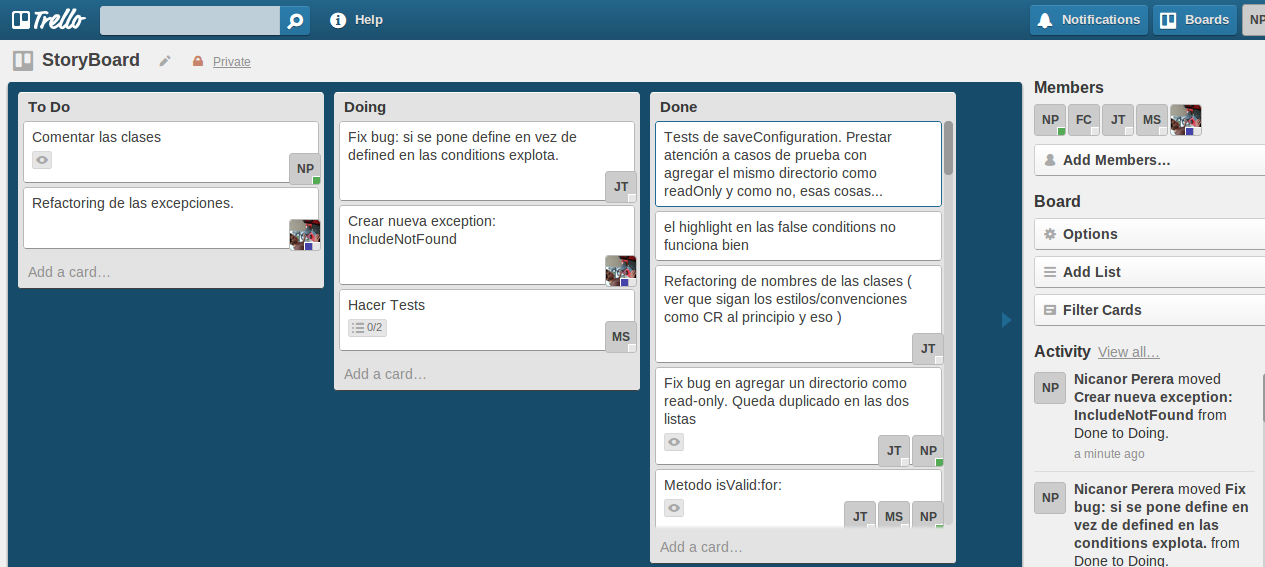
\includegraphics[scale=0.27]{images/trello.png}
    \caption{StoryBoard de Trello}
    \label{trello}
\end{figure}

\section{Testing}
\label{sec:testing}
Para poder minimizar la posibilidad de que alg\'un error fuera introducido durante el proceso de desarrollo el equipo tom\'o dos desiciones arquitect\'onicas. La primera fue practicar Test-driven development (TDD), lo que implica que ante cada nueva funcionalidad agregada deb\'iamos implementar la  nueva interface del objeto para inmediatamente despu\'es realizar un caso de prueba utilizando tests de unidad que probar\'an dicha interface, la historia de usuario asociada a dicha implementaci\'on no ser\'ia entonces terminada hasta que el test case pasase exitosamente. En segundo lugar dado que gran parte de nuestro aporte a CRefactory fue el de la implementaci\'on de parte de la interfaz gr\'afica de usuario se decidi\'o que cada vez que se agregue un nuevo elemento a la misma se haga un testeo manual, tanto de la parte nueva como de el resto de la aplicaci\'on, el testo manual fue cuidadosamente planificado para que \'este fuera fielmente reproducible y poder asegurar que la interface siempre fuese testeada de la misma manera, garantizando el perfecto funcionamiento de la interface.
\'Estas decisiones fueron tomadas basadas en que el contar con casos de prueba para cada funcionalidad individual genera confianza en el c\'odigo escrito, ante cada cambio o refactoring se tiene seguridad en que si las pruebas pasan la implementaci\'on es correcta.


\section{Frameworks y herramientas utilizadas}
\label{sec:frameworks_and_tools}
El proyecto est\'a implementado en Smalltalk, utilizando el entorno de desarrollo VisualWorks. Smalltalk es un lenguaje de programaci\'on orientado a objetos y de tipado din\'amico mientras que VisualWorks es una implementaci\'on multiplataforma de este lenguaje.

Para realizar los tests de unidad utilizamos el framework SUnit.

\subsection{CRefactory}
CRefactory es un herramienta para realizar refactorizaci\'on de c\'odigo C de forma autom\'atica utilizando una interfaz gr\'afica.

La refactorización del software es una parte importante del proceso de desarrollo de software, especialmente en la fase de mantenimiento. La refactorización es acerca de modificar software para que sea fácil de entender y cambiar, teniendo en cuenta que las modificaciones no alteran el comportamiento externo del software, sino que sólo comprende la manipulación sintáctica.


\subsection{Clases principales}

A continuacion se explican las clases principales de la interfaz de CRefactory. En la figura ~\ref{diagrama_de_clases_2} se puede ver un diagrama de Clases simplificado.

\begin{figure}[h!]
  \centering
    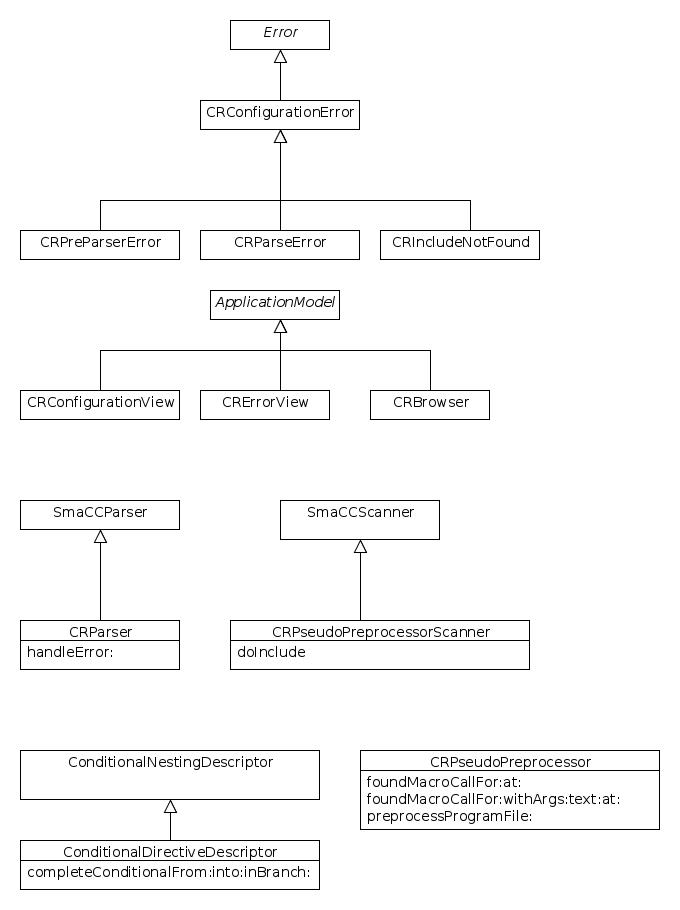
\includegraphics[scale=0.58]{images/diagrama_de_clases3.jpg}
    \caption{Diagrama de clases}
    \label{diagrama_de_clases_2}
\end{figure}

\begin{description}
\item[CRBrowser] Esta clase representa la ventana principal de la interfaz.

\item[CRConfigurationView] En esta clase esta imeplementada la interfaz para la gesti\'on de la configuraci\'on.

\item[CRErrorView] Esta clase se encarga se encarga de mostrar los mensajes de error cada vez que se produce una excepci\'on.

\item[CRConfigurationError] Esta es la clase base para el manejo de las excepciones. Aqu\'i se tienen datos como el archivo en el que se produjo el error o el n\'umero de l\'inea.

\item[CRPreparserError] Aqu\'i se manejan las excepciones producidas por errores en el preparser.

\item[CRParseError] Aqu\'i se manejan las excepciones producidas por errores en el parseo del c\'odigo fuente.

\item[CRIncludeNotFound] Aqu\'i se manejan las excepciones producidas por no haber encontrado una cabecera necesario.

\end{description}

\subsection{Funcionabilidades B\'asicas}

En la figura ~\ref{diagrama_de_secuencia_include_not_found} mostramos, a modo de ejemplo, un diagrama de secuencia simplificado del proceso de preprocesamiento para el caso en que no se encuentre alguno de los directorios de inclusión.

\begin{figure}[htbp]
  \centering
  \setlength{\unitlength}{\textwidth} 
    \begin{picture}(1,0.5)
       \put(-0.2,0){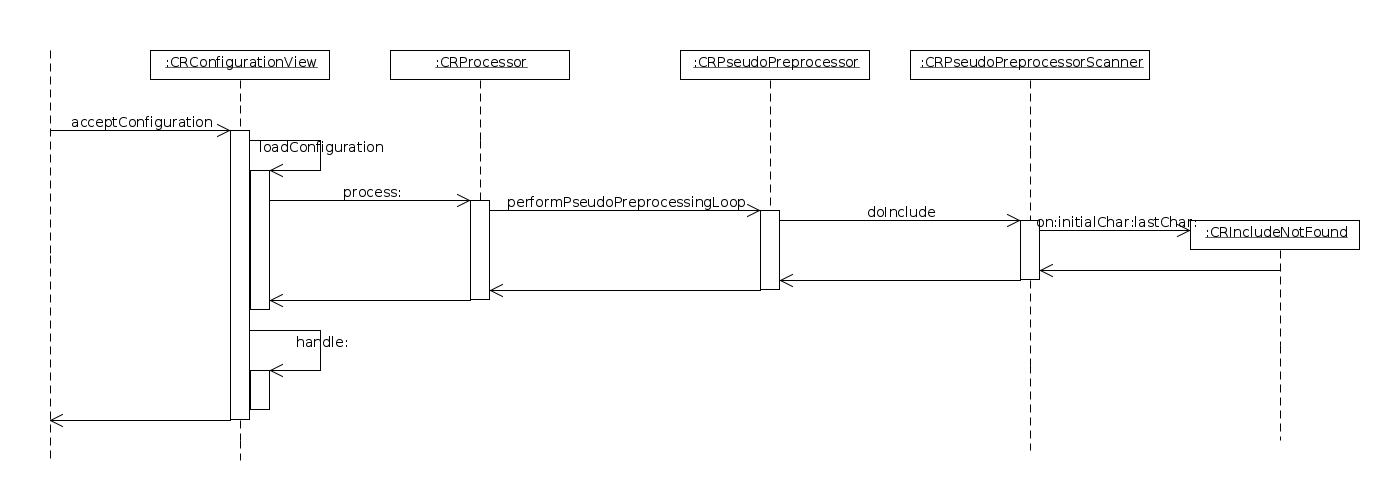
\includegraphics[width=1.4\unitlength]{images/secuencia_include_not_found.jpg}}
    \end{picture}
    \caption{Diagrama de Secuencia de directorio de inclusión no encontrado}
    \label{diagrama_de_secuencia_include_not_found}
\end{figure}

La figura ~\ref{diagrama_de_secuencia_parser_error} se corresponde con un diagrama de secuencia en el que se explica lo que sucede en caso de un error de parseo.

\begin{figure}[htbp]
  \centering
  \setlength{\unitlength}{\textwidth} 
    \begin{picture}(1,0.5)%in case your image is twice as wide as it is high
                          %(otherwise change the 0.5 to your file's height/width).
       \put(-0.2,0){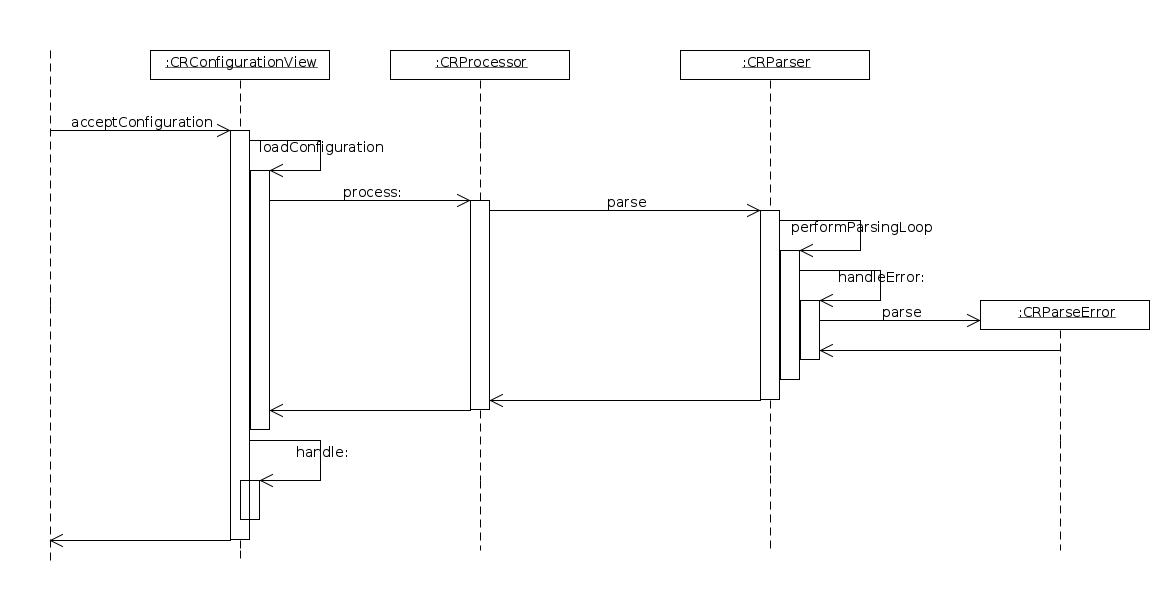
\includegraphics[width=1.4\unitlength]{images/secuencia_parser_error.jpg}}
    \end{picture}
    \caption{Diagrama de Secuencia de error de parseo}
    \label{diagrama_de_secuencia_parser_error}
\end{figure}

\clearpage

\section{Problema uno: Carga de archivos}
\label{sec:problema_uno}

El primer paso para trabajar con CRefactory es seleccionar los archivos de c\'odigo C al cual se le va a aplicar la refactorizaci\'on y los directorios donde se encuentran los archivos de cabecera que incluyen dichos archivos.

Un archivo de cabecera es un archivo que el preprocesador incluye autom\'aticamente dentro del c\'odigo fuente del archivo que lo incluye. Estos archivos contienen normalmente una declaraci\'on directa de estructuras, funciones, variables u otros identificadores.


\subsection{Contexto}
Originalmente se deb\'ia especificar manualmente la ruta absoluta donde se localizaban el o los archivos que se deseban incluir (Figura ~\ref{carga_original}). Esto no es adecuado ya que se podr\'ian cometer errores de tipeo o incluso no recordar exactamente cual era la ruta deseada.
Al cometer un error de tipeo o escribir el nombre de un archivo inexistente ocurr\'ia un error como el de la Figura ~\ref{error}.

\begin{figure}[h!]
  \centering
    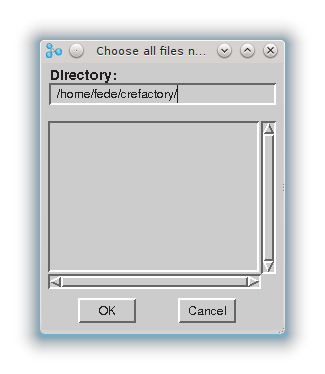
\includegraphics[scale=0.85]{images/codigo_original/carga.png}
    \caption{Carga de archivo original}
    \label{carga_original}
\end{figure}

\begin{figure}[h!]
  \centering
    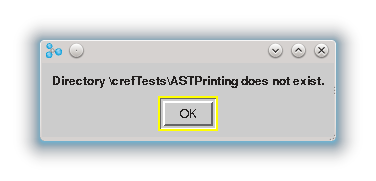
\includegraphics[scale=0.85]{images/codigo_original/error.png}
    \caption{Error}
    \label{error}
\end{figure}

\subsection{Soluci\'on planteada}
El problema fue solucionado agregando un di\'alogo de exploraci\'on de archivos, tanto para la selecci\'on de los ficheros a editar como para la especificaci\'on de el/los directorio/s donde se encuentran los archivos de cabecera. El di\'alogo permite inspeccionar el filesystem y seleccionar el archivo deseado eliminando as\'i la necesidad de tener que recordarse cual era la ubicaci\'on del archivo deseado y al mismo tiempo excluyendo la posibilidad de que la ruta sea erronea. Adem\'as, esta aproximaci\'on permite seleccionar m\'as de un archivo al mismo tiempo.

En la Figura~\ref{carga_archivo} se muestra un pantallazo de la visualizaci\'on de la nueva ventana de carga archivos y en la Figura~\ref{busqueda_archivo} el di\'alogo de exploraci\'on del filesystem.

\begin{figure}[h!]
  \centering
    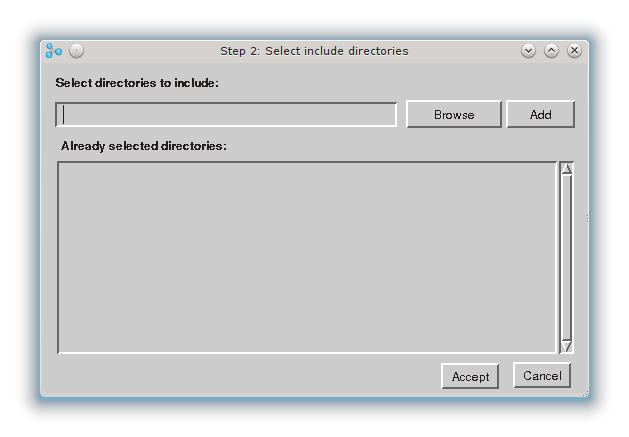
\includegraphics[scale=0.50]{images/codigo_modificado/include.png}
     \caption{Carga de archivo}
     \label{carga_archivo}
\end{figure}

\begin{figure}[h!]
  \centering
    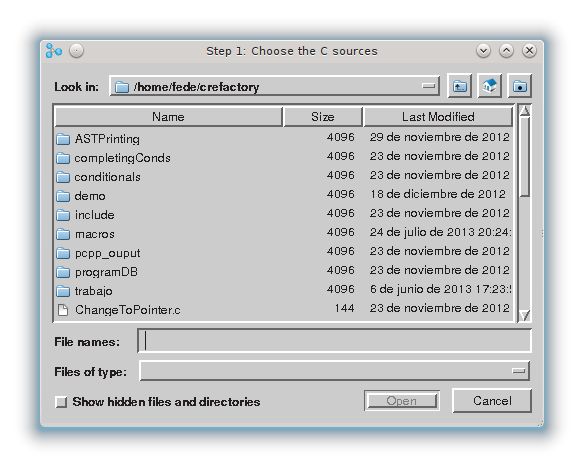
\includegraphics[scale=0.50]{images/codigo_modificado/open_file.png}
     \caption{Exploraci\'on del filesystem}
     \label{busqueda_archivo}
\end{figure}

\section{Problema dos: Configuraci\'on}
\label{sec:problema_dos}

Un archivo fuente de c\'odigo C no s\'olo contiene sintaxis del lenguaje, sino que puede, y suele, contener directivas al preprocesador, tales directivas brindan la posibilidad de realizar inclusi\'on de archivos (como los archivos cabecera), definici\'on de macros o compilaci\'on condicional.

Una macro es una forma de sustituir caracteres por otros, las macros constan de un nombre y un cuerpo, durante el preprocesado cada ocurrencia del primero ser\'a reemplazado por el segundo. El cuerpo de la macro puede referir directamente a elementos globales del programa o hacerlo indirectamente, a trav\'es de la concatenaci\'on de s\'imbolos, lo que puede f\'acilmente violar la correctitud de una refactorizaci\'on.

La compilaci\'on condicional proporciona una forma de incluir c\'odigo selectivamente dependiendo del valor de determinadas condiciones en tiempo de compilaci\'on, lo que puede derivar en m\'ultiples ramas que son mutuamente exclusivas, si durante una refactorizaci\'on s\'olo se considera una de ellas las otras pueden volverse obsoletas o erroneas y si por el contrario todas las ramas son consideradas cada elemento puede tener m\'ultiples definiciones, como una variable con m\'ultiples tipos.

Dado que la herramienta CRefactory puede realizar operaciones de refactorizaci\'on sobre c\'odigo sin preprocesar es necesario otorgarle cierta informaci\'on extra que le permita a la herramienta resolver situaciones dificiles de manejar a la hora de refactorizar, \'esta informaci\'on es llamada configuraci\'on. En concreto la configuraci\'on necesaria es:

\begin{itemize}
\item Directorios d\'onde se encuentran los archivos incluidos por el archivo cargado.
\item Cuerpos de macros.
\item Condiciones falsas para determinar que ramas de c\'odigo deben ser tenidas en cuenta y cuales no a la hora de refactorizar.
\end{itemize}

\subsection{Contexto}
La interfaz de CRefactory permit\'ia, como se dijo en la secci\'on~\ref{sec:problema_uno}, ingresar los directorios donde se alojan los archivos incluidos por el archivo a editar, pero no brindaba la posibilidad de definir cuerpos de macros ni de especificar condiciones falsas por lo cual era necesario extender la GUI para proveer esa funcionalidad.

\subsection{Soluci\'on planteada}
Se decidi\'o implementar una nueva ventana que servir\'ia de interfaz para ingresar la informaci\'on de configuraci\'on. Dado que ya exist\'ian dos ventanas de di\'alogo para realizar parte de la configuraci\'on (la selecci\'on de los archivos fuente a editar y la especificaci\'on de la ubicaci\'on de los archivos incluidos por dichos fuentes) se opt\'o por no sobrecargar la vista agregando un di\'alogo m\'as, o quiz\'as incluso m\'as de uno teniendo en cuenta que se necesitaba brindar la posibilidad de definir tanto macros como condiciones falsas, sino unificar todos estos aspectos relacionados en una sola vista. Por \'ultimo nos inclinamos a utilizar una vista  con solapas dado que una sola ventana con tanta informaci\'on podr\'ia resultar confusa y se dificultar\'ia encontrar r\'apidamente d\'onde ingresar la informaci\'on de configuraci\'on deseada, por otro lado mucha de esa informaci\'on s\'olo ser\'a necesaria en algunos casos, por ejemplo muchas veces se podr\'a editar un archivo donde no fuera necesario definir macros, por lo que la vista en solapas se ajusta a la necesidad de s\'olo mostrar lo necesario y no m\'as que eso, quien no necesite definir macros puede simplemente obviar esa solapa.

El resultado final fue entonces el mostrado en la Figura~\ref{configuracion}.

\begin{figure}[h!]
  \centering
    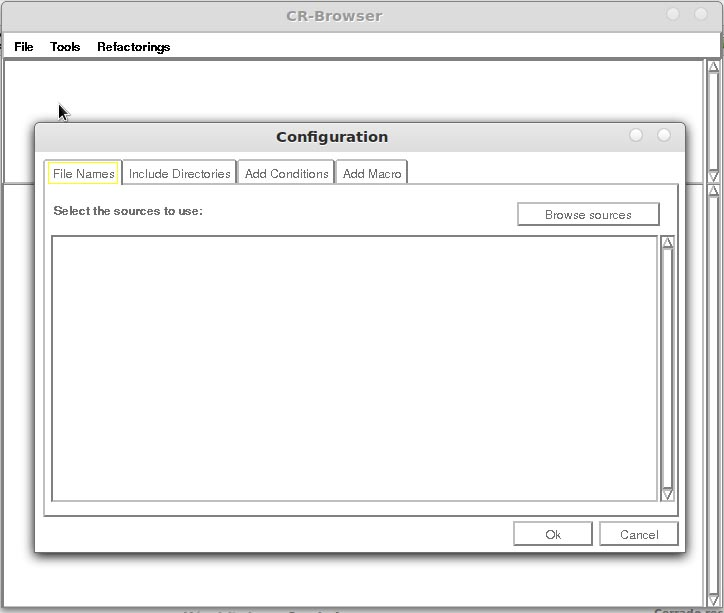
\includegraphics[scale=0.45]{images/codigo_modificado/configuracion.jpg}
     \caption{Interfaz de configuraci\'on}
     \label{configuracion}
\end{figure}

\section{Problema tres: Manejo de excepciones}

El manejo de excepciones es una t\'ecnica de programaci\'on que permite controlar los errores ocasionados durante la ejecuci\'on del programa.
A continuaci\'on se detallan los problemas que presentaban la ausencia del manejo de estas en la interface de CRefactory y como fueron solucionados estos problemas.

\subsection{Contexto}
Ante un error la aplicaci\'on generaba una excepci\'on pero \'esta no era manejada por lo cual la herramienta dejaba de funcionar. No hab\'ia ning\'un tipo de manejo de excepciones. No encontrar un archivo de cabecera en los directorios incluidos significaba que el programa se cerrara abruptamente, sin ning\'un tipo de retroalimentaci\'on para que el usuario pueda rastrear el error. Se hizo evidente la necesidad de que el usuario pudiera rastrear el error y corregirlo sin que falle la herramienta.

\begin{figure}[h!]
  \centering
    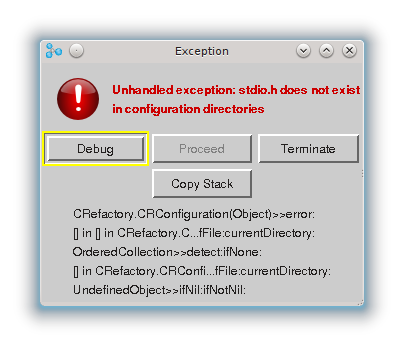
\includegraphics[scale=0.85]{images/codigo_original/error_header_no_agregado.png}
     \caption{Error por header no incluido}
     \label{header_no_incluido}
\end{figure}

\subsection{Soluci\'on planteada}
Lo que se hizo en un principio fue implementar los manejadores para las excepciones. Por lo que cuando se produc\'ia una excepci\'on se mostraba una ventana con una descripci\'on del error ayudando al usuario para que puediera corregirlo. Por ejemplo, cuando no se inclu\'ia el directorio donde buscar una cabecera se mostraba una ventana que advert\'ia al usuario del error y le daba la posibilidad de corregirlo agregando el directorio necesario en la ventana de configuraci\'on.

En la Figura ~\ref{header_no_encontrado} se ve como se mostraba el error luego de implementar el manejo de excepciones.

\begin{figure}[h!]
  \centering
    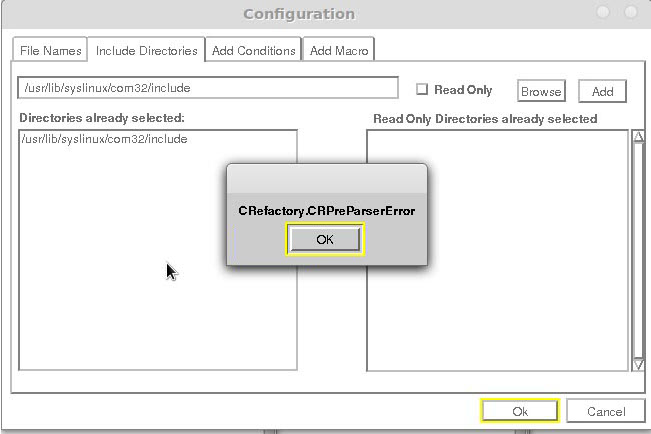
\includegraphics[scale=0.50]{images/codigo_modificado/error_header_no_encontrado_sin_view_error.jpg}
     \caption{Error por header no encontrado}
     \label{header_no_encontrado}
\end{figure}

\section{Problema cuatro: Ventana de error}

Al ocurrir una exepci\'on no hab\'ia manera de que el usuario pudiera tratarla. Se vio la necesidad de visualizar el problema gr\'aficamente a trav\'es de una ventana de error

\subsection{Contexto}
El problema de la soluci\'on planteada en el punto anterior es que no mostraba en que parte del c\'odigo fuente se produjo el error. Por lo tanto el usuario no siempre pod\'ia recuperarse totalmente.

\subsection{Soluci\'on planteada}
\'Esto llev\'o a reemplazar la ventana de notificaci\'on de error por una que diera la posibilidad de visualizar el c\'odigo fuente informando el error que se produjo. En la Figura ~\ref{ventana_de_error} se muestra una imagen de la ventana mostrando el error.

\begin{figure}[h!]
  \centering
    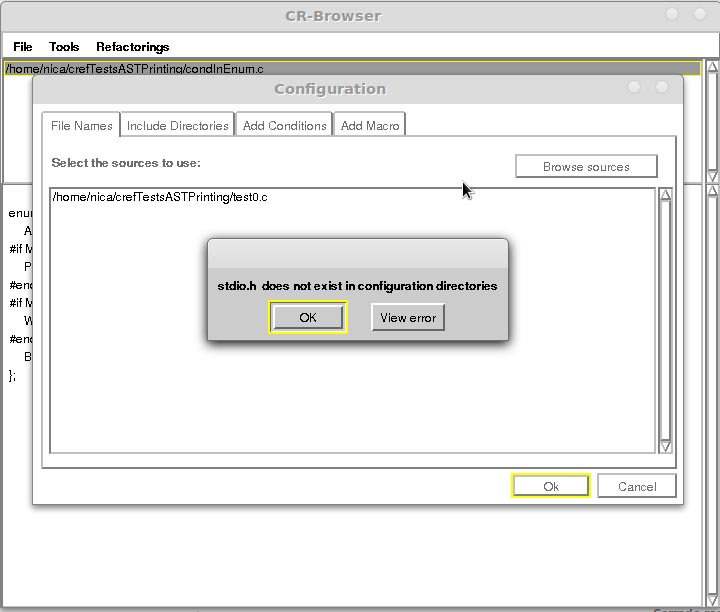
\includegraphics[scale=0.50]{images/codigo_modificado/error_header_no_encontrado.jpg}
     \caption{Ventana de error}
     \label{ventana_de_error}
\end{figure}

La ventana de error deb\'ia ser capaz de mostrar toda la informaci\'on posible acerca del error producido, por ejemplo la l\'inea de c\'odigo que lo ocacion\'o, o el nombre de un archivo que haya sido incluido y sin embargo no pudo ser encontrado. Para lograr \'esto se implement\'o una serie de clases que extendieran el framework de colecciones de VisualWorks y que puedieran representar fielmente al error ocurrido siendo capaces de brindar la informaci\'on \'util de cada uno, estas clases ser\'ian entonces levantadas como excepciones cuando un error fuera producido. Dichas clases forman entonces una jerarqu\'ia, heredando todas de la clase base CRConfigurationError, esta \'ultima clase no s\'olo agrupa funcionalidad com\'un sino que define algunos m\'etodos abstractos que deben ser implementados por las subclases, especificando as\'i una API y garantizando que la ventana de error pudiera manejar todas las excepciones y conseguir toda la informaci\'on necesaria para ser mostrado haciendo uso de esa API.
En la Figura~\ref{diagrama_clases_excepciones} se muestra la jerarqu\'ia de clases implementadas y como heredan de Error, clase base dentro del framework de excepciones de VisualWorks.

\begin{figure}[h!]
  \centering
    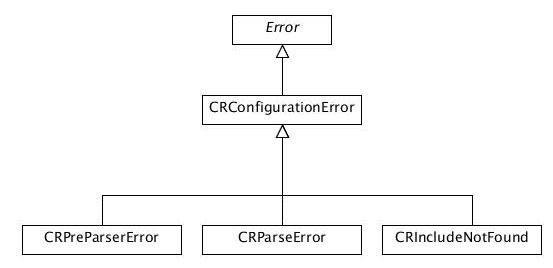
\includegraphics[scale=0.6]{images/diagrama_clases_excepciones.jpg}
    \caption{Jerarqu\'ia de excepciones}
    \label{diagrama_clases_excepciones}
\end{figure}

\section{Problema cinco: Highlight del error}

Cuando ocurre un error es \'util conocer que l\'inea o l\'ineas de c\'odigo son las que lo provocaron. Para poder identificar una porci\'on de c\'odigo, estuvimos de acuerdo en que ser\'ia muy \'util contar con alg\'un tipo de resaltado de texto.

\subsection{Contexto}
Anteriormente, luego de un error se mostraba el c\'odigo pero no era claro que l\'ineas lo hab\'ian producido. Esto era un problema ya que la idea del manejo de excepciones no es solo identificar el error sino encontrar la manera de solucionarlo. Y muchas veces para solucionar un problema es necesario saber exactamente en que porci\'on del c\'odigo se origin\'o.

\subsection{Soluci\'on planteada}
El problema se solucion\'o implementando en la interfaz el resaltado de las l\'ineas donde se produjo el error. Gracias a esto el programador puede solucionar los errores con mucha mayor facilidad.

En la Figura ~\ref{resaltado} se visualiza el resaltado de un error.
\begin{figure}[h!]
  \centering
    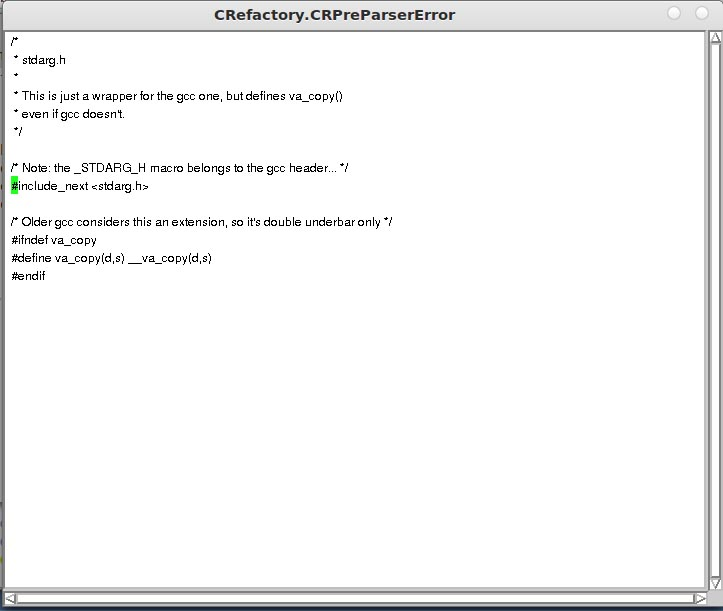
\includegraphics[scale=0.50]{images/codigo_modificado/highlight_preparser.jpg}
     \caption{Resaltado del error}
     \label{resaltado}
\end{figure}


\section{Instrucciones de instalaci\'on}

\begin{enumerate}
\item Instalar VW7.8nc
\item Abrir la imagen, guardarla con nuevo nombre y setear el VisualWorks home directory

\item Desde el Parcel Manager cargar:
  \begin{itemize}
  \item All Advanced Tools
  \item RBSUnitExtensions
  \end{itemize}
  
\item Conectarse al repositorio Store de la c\'atedra: catedras.lifia.info.unlp.edu.ar:5432\_tpoo y buscar entre los “Published Items” el Bundle CRefactory. Instalar la \'ultima versi\'on (1.4) y luego instalar el bundle CRefactoryGUI.

\item Lo siguiente es probar que los tests de CRefactory pasen correctamente. Estos tests crean archivos .c de prueba en un directorio que deben especificar. Para esto browsear el c\'odigo de: “CRefactory-Testing-Root”, clase “CREFTestCase”, m\'etodo de clase “codeDirectory” y editarlo haciendo referencia a un directorio ya creado en la m\'aquina.
  
\item Seleccionar el package {\it CRefactory-Testing} y correr todos los tests. Deber\'ian pasar los 173 tests.

\item Para correr la aplicaci\'on debemos ejecutar en el \'area de trabajo  {\it CRBrowser open}. 
\end{enumerate}

\section{Instrucciones de uso}

Una vez abierta la aplicación, se nos aparecerá la ventana principal de la aplicación, la cual se divide en dos secciones. En la sección ubicada en la parte superior se ubican los archivos a los cuales se les está aplicando refactoring. Al hacer click en el nombre de un archivo, se visualiza su código en la sección inferior. [Figura ~\ref{inicio}].

\begin{figure}[h!]
  \centering
    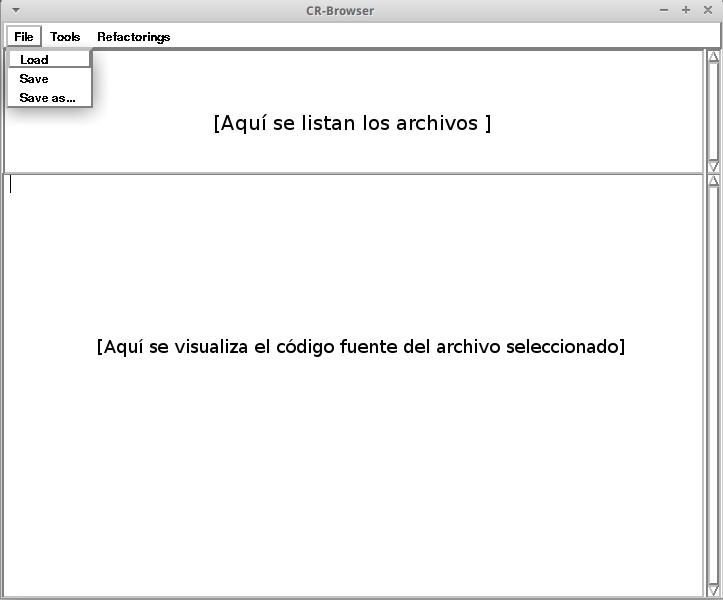
\includegraphics[scale=0.50]{images/uso/inicio.jpg}
     \caption{Ventana principal}
     \label{inicio}
\end{figure}

Al seleccionar File - Load, se abrirá una ventana con cuatro pestañas. 

En la primer pestaña se debe seleccionar el o los archivos a los cuales se les quiere realizar refactoring. Se puede escribir el path del archivo, o seleccionarlo haciendo click en el botón "Browse Sources". Se puede seleccionar más de un archivo. [Figura ~\ref{file_names}].

\begin{figure}[h!]
  \centering
    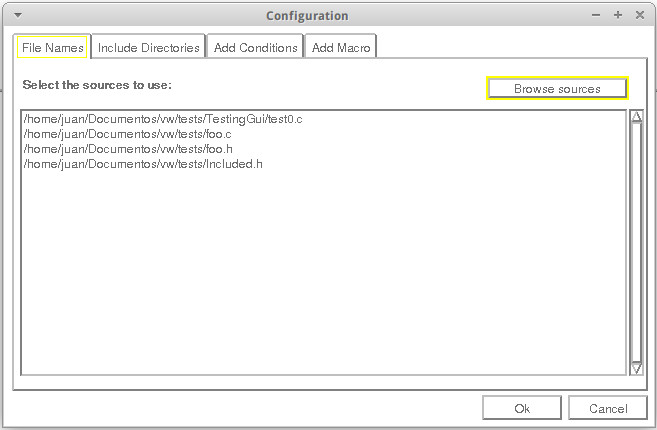
\includegraphics[scale=0.50]{images/uso/file_names.jpg}
     \caption{Selecci\'on de archivos}
     \label{file_names}
\end{figure}

En la segunda pestaña se pueden seleccionar las carpetas en las cuales se encuentran los directorios de inclusión. Ésto es necesario para poder realizar refactoring a archivos con include directories. Un directorio se puede marcar como de Sólo Lectura si es necesario, haciendo click en el checkbox "Read Only". Los directorios de sólo lectura se mostrarán en el listado de la derecha, mientras que el resto se mostrarán en el listado de la izquierda. [Figura ~\ref{include_directories}].

\begin{figure}[h!]
  \centering
    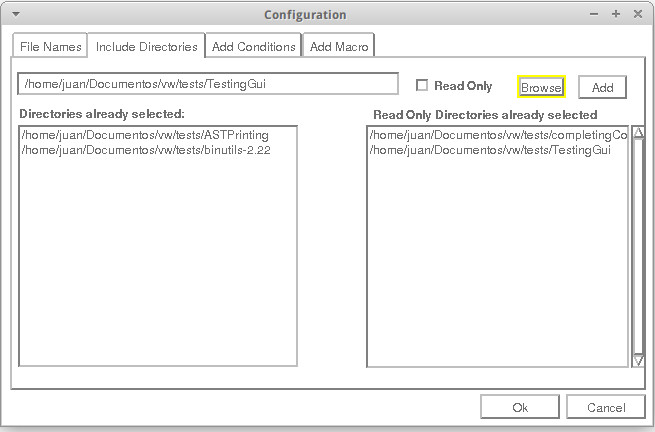
\includegraphics[scale=0.50]{images/uso/include_directories.jpg}
     \caption{Selecci\'on de directorios}
     \label{include_directories}
\end{figure}

En la tercer pestaña se pueden agregar condiciones falsas y en la cuarta pestaña se pueden agregar macros.

Una vez seleccionadas todas las opciones necesarias, en caso de que no ocurra ningún error de configuraci\'on, se volver\'a a la ventana principal y se podrá refactorizar el c\'odigo. A modo de ejemplo mostramos en la Figura ~\ref{rename} c\'omo se podr\'ia aplicar el renombramiento de una variable.

\begin{figure}[h!]
  \centering
    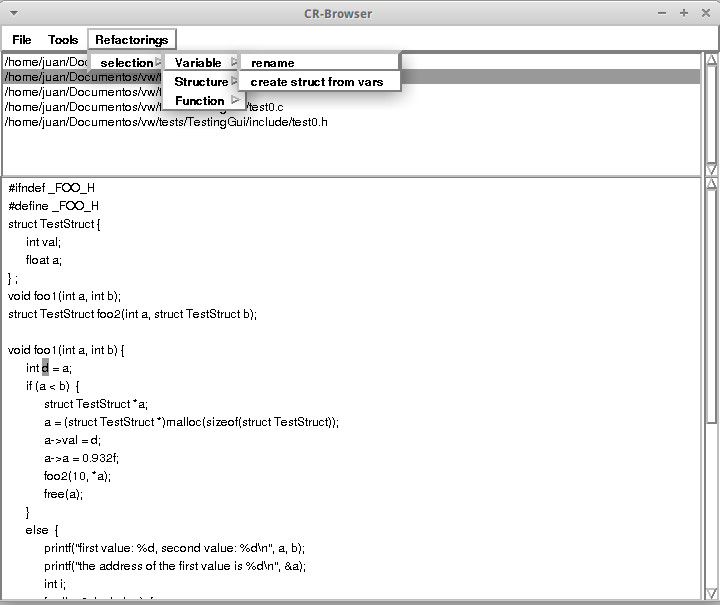
\includegraphics[scale=0.50]{images/uso/rename.jpg}
     \caption{Ejemplo de refactorizaci\'on}
     \label{rename}
\end{figure}

\clearpage

\section{Minutas}
\label{sec:minutas}
Durante el desarrollo del proyecto tuvimos varias reuniones con la Profesora, con la finalidad de conocer cu\'ales eran los requerimientos y mostrar el avance del proyecto. Cada vez que ten\'iamos una reuni\'on deb\'iamos tomar apuntes de lo que hab\'iamos hablado.

A continuaci\'on presentamos dichos apuntes o minutas:

\subsection{Reuni\'on del Lunes 10/09}
La Profesora nos di\'o una breve introducci\'on al proyecto y un vistazo general de c\'omo est\'a organizado. Nos explic\'o c\'omo estaba funcionando hasta ese momento. Aprendimos c\'omo cargar el proyecto dentro de visualworks y a realizar todas las configuraciones necesarias para el correcto funcionamiento de la aplicaci\'on.

Nos explic\'o c\'omo conectarnos al repositorio de la c\'atedra y c\'omo utilizar la herramienta de control de versiones.
Acordamos que nos enviar\'ia por correo electr\'onico los nombres de usuarios y contraseñas de cada integrante del grupo para acceder al repositorio.

Luego de esta introducci\'on al proyecto hablamos las funcionalidades que tendr\'iamos que implementar a lo largo de la cursada. Las m\'as importantes:

\begin{itemize}
  \item Mejorar el di\'alogo de carga de un archivo. Que sea por ejemplo como el de carga de parcels, haci\'endolo m\'as accesible al usuario.
  \item Poder especificar donde est\'an los directorios con los archivos de cabecera.
  \item Tener en cuenta las configuraciones que no se pueden parsear.
  \item Manejar las excepciones para que cuando hay una configuraci\'on inv\'alida muestre en el c\'odigo donde est\'a lo inv\'alido. 
\end{itemize}

Adem\'as se coment\'o que ser\'ia interesante como trabajo a futuro, posibilitar la creaci\'on autom\'atica de grafos de la inclusi\'on de archivos.

\subsection{Reuni\'on del Lunes 17/09}
En esta reuni\'on la Profesora nos enseñ\'o c\'omo funcionaba el di\'alogo de carga de archivos. Anteriormente era necesario escribir el nombre de los archivos a incluir, lo cual hac\'ia tedioso el trabajo y ocurr\'ia que ante un error de tipeo no se encontrar\'ia el archivo y el programa cerrar\'ia abruptamente. 

Planteamos modificar el di\'alogo de carga de archivo para que permita explorar el filesystem. De esta manera ser\'ia m\'as f\'acil de utilizar y se solucionar\'ian los problemas.

\subsection{Reuni\'on del Jueves 18/10}
Para este momento ya hab\'iamos implementado la carga de archivos y directorios por medio de un File Browser, pero todav\'ia no era el ideal.

En esta reuni\'on se habl\'o con la Profesora sobre la necesidad de marcar a algunos directorios como directorios de s\'olo lectura (Read Only).

Tambi\'en hablamos sobre la implementaci\'on de manejo de excepciones. En particular ocurr\'ia frecuentemente una excepci\'on al no incluir los directorios necesarios. Acordamos implementar el manejo de dicha excepci\'on.


Adem\'as comentamos los siguientes puntos:
\begin{itemize}
 \item Mejorar la secci\'on include Directory, para que se puedan agregar directamente.
 \item Bajar un ejemplo opensource en C para probar el funcionamiento.
 \item Prestar atenci\'on a preprocess y a FullNameOfFile.
\end{itemize}

\subsection{Reuni\'on del Lunes 29/10}
En esta reuni\'on comenzamos a hablar sobre el tratamiento de excepciones en CRefactory. La Profesora nos aconsej\'o que leamos la documentaci\'on del manejo de excepciones en Visual Works y que mirar\'amos ejemplos en su c\'odigo fuente para elegir la estrategia a utilizar.

Cuando se produc\'ia un error, CRefactory no indicaba cu\'al era el archivo que lo hab\'ia producido. Nos propusimos como objetivo que se pueda mostrar dicho archivo, y resaltar la l\'inea de c\'odigo en la cu\'al se produjo el error.

\subsection{Reuni\'on del Lunes 12/11}
Durante la implementaci\'on de las diferentes funcionalidades, no tuvimos en cuenta el correcto funcionamiento de la aplicaci\'on, y descubrimos que algunas cosas hab\'ian dejado de funcionar. La Profesora nos sugiri\'o que nos asegur\'aramos de que pasen los tests de CRefactory. Nos propusimos realizar tests de todas las funcionalidades importantes que implement\'aramos.

Los errores de parseo en presencia de condiciones falsas sol\'ia ser un problema, ya que muchas veces se dificultaba encontrar el lugar donde ocurr\'ia el error. La Profesora plante\'o resolverlo y nos recomend\'o comenzar probando con el archivo test19.c.

\subsection{Reuni\'on del Jueves 29/11}
En esta reuni\'on volvimos a hablar acerca de los problemas vinculados con las condiciones falsas. Se nos pidi\'o tener la posibilidad de cachear la excepci\'on que ocurr\'ia al agregar una condici\'on falsa y se nos sugiri\'o investigar la implementaci\'on de la clase Preprocessor.

\section{Conclusiones}
\label{sec:conclusiones}
En esta secci\'on explicaremos los logros alcanzados durante el proyecto, los valores que obtuvimos y algunas sugerencias para un futuro trabajo de CRefacory.

\subsection{Logros alcanzados}
La nueva interfaz es pr\'actica para cargar archivos, directorios, macros y condiciones falsas. Ahora se pueden cargar archivos de forma segura. En lugar de escribir el nombre del archivo o directorio se lo puede seleccionar entre los ya existentes. 

Ahora es posible acceder a funcionalidades que antes no se pod\'ian, como por ejemplo la posibilidad de agregar condiciones falsas a la configuraci\'on para que no sean parseadas.

Cambiamos el diseño de la interfaz de manera que sea, a nuestro criterio, mucho m\'as amigable con el usuario.

Al dispararse una excepci\'on de parseo, la nueva interfaz ahora permite detectar la l\'inea de c\'odigo en la cual ocurri\'o.

\subsection{Valores obtenidos}
Trabajamos utilizando una metodolog\'ia \'agil de tipo Scrum. \'Esto nos permiti\'o tener una buena organizaci\'on. Ayud\'o al trabajo en equipo, optimiz\'o la eficiencia en la resoluci\'on de las tareas.

Comprendimos la importancia de realizar tests automatizados durante la programaci\'on. Si bien nos demor\'o implementar el c\'odigo de los tests, creemos que a la larga salimos beneficiados con respecto a la distribuci\'on del tiempo. Adem\'as saber que el programa segu\'ia funcionando nos daba mucha m\'as seguridad al programar.

\subsection{Trabajo futuro}
En orden de conseguir que CRefactory sea una herramienta profesional que pueda competir con otros productos similares creemos que se debe soportar las siguientes caracter\'isticas:

\subsubsection{Coloreado de Sintaxis}
El coloreado de sintaxis es una caracter\'istica muy com\'un en los editores de texto modernos, consiste en mostrar el c\'odigo fuente en diferentes colores con el objetivo de mejorar la legibilidad del c\'odigo para el programador.

\subsubsection{Localizaci\'on autom\'atica de c\'odigo refactorizable}
Actualmente, para refactorizar c\'odigo, el programador debe identificar el problema observando el c\'odigo. Creemos que ser\'ia buena idea implementar un algoritmo que sirva para localizar c\'odigo potencialmente refactorizable de manera autom\'atica.

\subsubsection{Integraci\'on con frameworks de testing}
Al refactorizar c\'odigo, debemos comprobar que el c\'odigo siga funcionando correctamente. Ser\'ia deseable que CRefactoring tenga integrados frameworks de testing para realizar el testeo del c\'odigo de forma autom\'atica.

\subsubsection{Personalizaci\'on del entorno}
Ser\'ia bueno otorgar a la interface cierta flexibilidad para poder adaptarse a las necesidades de cada usuario.


\subsubsection{Formateo autom\'atico de c\'odigo}
El formateo de c\'odigo es una herramienta que permite modificar el c\'odigo para que \'este se presente siguiendo convenciones de identaci\'on, espaciado y posicionamiento. \'Esto ayuda a que el c\'odigo sea m\'as f\'acil de leer, entender y mantener para el desarrollador.

Creemos que ser\'ia ideal que CRefactory cuente con una herramienta de formateo autom\'atico.


\subsubsection{Tabla de s\'imbolos}
Una tabla de s\'imbolos es una estructura de datos donde cada s\'imbolo en el c\'odigo fuente de un programa est\'a asociado con informaci\'on, como por ejemplo la ubicaci\'on, el tipo de datos y el \'ambito de cada variable.

Ser\'ia bueno poder ver la tabla de s\'imbolos.

\subsubsection{Grafo de dependencias}
Puede ser \'util visualizar las dependencias del c\'odigo fuente. Ser\'ia interesante contar con una herramienta que realice grafos de inclusi\'on de archivos de forma autom\'atica.

\end{document}